%#! platex  -halt-on-error -file-line-error -src-specials main.tex
% Time-stamp: <2017-01-20 17:59:34 takago2>

% 基本設定 =====================================
\documentclass[9pt,dvipdfmx]{jsarticle}
\usepackage{graphicx}
\usepackage[top=15truemm,bottom=15truemm,left=20truemm,right=20truemm]{geometry}
\pagestyle{empty}
\usepackage[deluxe]{otf}
\doublerulesep=\arrayrulewidth
\setlength\intextsep{0pt}
\setlength\floatsep{0pt} %dblfloatsep
\setlength\textfloatsep{0pt} %dbltextfloatsep
\renewcommand{\baselinestretch}{0.8}

%-----------------------------------------------------
% 見出し上下の余白などの調整 from here
\makeatletter
\def\section{\@startsection {section}{1}{\z@}
{1ex plus -1ex minus-.2ex}%余白上
{0ex plus 1.2ex}%余白した
 {\normalsize\bf}%体裁
 }
\def\subsection{\@startsection {subsection}{1}{\z@}
{1ex plus -1ex minus-.2ex}%余白上
{0ex plus 1.2ex}%余白下
 {\normalsize\bf}%体裁
 }
\makeatother
% section/subsectionの調整
\renewcommand{\thesection}{\arabic{section}.\hskip-9pt}
\renewcommand{\thesubsection}{\arabic{section}.\arabic{subsection}.\hskip-9pt}
% 見出しの調整 end here
%-----------------------------------------------------
%
\renewcommand{\refname}{\underline{参考文献}} 
\begin{document}
% タイトル =====================================
\twocolumn[
\vspace{-5mm}
\begin{flushright}
\large \bfseries{EP999}
\end{flushright}
\begin{center}
{\large 最小自乗法を用いた画素ごとの局所適応予測符号化法}\vspace{2mm}
\end{center}
% 著者情報 =====================================
\begin{minipage}{185mm}
\begin{center}
{
担当者: {武田 晴信},{武田 信繁},{武田 信廉}
\hspace{1cm}
指導教員:{鷹合 大輔}
}
\end{center}
\end{minipage}
\vspace{3mm}
] 
% 本文  =========================================
\section{\underline{はじめに}}
画像の予測符号化において最小自乗法を用いて,ブロックごと又は画素ごとに予測式係数を決定する手法が提案されている)\cite{sdkguide}.ブロックごとに予測式係数を決定する方法では,そのブロック内の全ての画素を使って予測誤差の自乗和を最小化する予測式係数を決定するが,符号化(復号化)が済んでいない画素を利用しているために,予測式係数をブロックごとに伝送せねばならず,高次予測をするとブロックごとのオーバヘッドが増加してしまう.また,画素ごとに予測式係数を決定する方法では,予測式係数は符号化(復号化)が済んだ領域を使って決定するため,オーバヘッドは増えないが,符号化効率が高くない.そこで,著者らは画素ごとに予測式係数を決定するが,予測式の形状と参照領域サイズをブロックごとに決定する方法を試みた結果,少ないオーバヘッドでも効果が見られたので報告する.
% section 2 ----
\section{\underline{ブロックごとに予測式形状と参照領域サイズを選択する方法}}
画素ごとに予測を行う場合は,比較的高次(12次以上)が効果的であるが,局所的には,低次予測が適当な場合がある.そこで画素ブロック$b$に対して,予測誤差の自乗和
$$
S_b(p,L)=\sum_{n=0}^{N-1} \left\{ x_b(n)-\hat{x_b}_{p,L}(n) \right\}^2
$$
を最小化する予測式の形状$p$(Figure \ref{takago-paper2008080800268-fig:1}を参照)と,予測式係数を決定の為の参照領域サイズ$L$(Figure \ref{takago-paper2008080800268-fig:2}を参照)を見つけ,誤差系列とともに伝送する.ここで$n=0,1,2\cdots,N-1$は$b$内の画素番号,$x_b(n)$は画素値,$\hat{x_b}_{p,L}(n)$は予測値である.

本研究ではブロックサイズは$16\times16$,$32\times32$画素を1ブロックとして実験を行い,また$L$は符号化(復号化)が済んでいる画素であれば,ブロック境界を越えたものを使う.尚,簡単の為,画像の範囲外は画素値128と仮定しており,更に数値計算が不安定な画素に対しては予め用意しておいた固定式を用いた.

あああああああああああああああああああああああああああああああああああああfdっっっっっっっっっっっっっっっっs2134143412412341234qうぇrqうぇqうぇrqうぇrqうぇrqうぇrqうぇrqwえrとぇrとぇrとぇrてwrとぇrとぇrtごとに6ビット必要である.したがって,$16\times 16$,$32\times 32$[画素/ブロック]の場合,それぞれ約0.023[bpp],約0.006[bpp]がオーバヘッドとなる.バヘッドについては$p$が6種,$L$が10種であるので,1ブロックごとに6ビット必要である.したがって,$16\times 16$,$32\times 32$[画素/ブロック]の場合,それぞれ約0.023[bpp],約0.006[bpp]がオーバヘッドとなる

また,オーバヘッドについては$p$が6種,$L$が10種であるので,1ブロックごとに6ビット必要である.したがって,$16\times 16$,$32\times 32$[画素/ブロック]の場合,それぞれ約0.023[bpp],約0.006[bpp]がオーバヘッドとなる.また,オーまた,オーバヘッドについては$p$が6種,$L$が10種であるので,1ブロックごとに6ビット必要である.したがって,$16\times 16$,$32\times 32$[画素/ブロック]の場合,それぞれ約0.023[bpp],約0.006[bpp]がオーバヘッドとなる.また,オーバヘッドについては$p$が6種,$L$が10種であるので,1ブロックごとに6ビット必要である.したがって,$16\times 16$,$32\times 32$[画素/ブロック]の場合,それぞれ約0.023[bpp],約0.006[bpp]がオーバヘッドとなる.また,オーバヘッドについては$p$が6種,$L$が10種であるので,1ブロックごとに6ビット必要である.したがって,$16\times 16$,$32\times 32$[画素/ブロック]の場合,それぞれ約0.023[bpp],約0.006[bpp]がオーバヘッドとなる.また,オーバヘッドについては$p$が6種,$L$が10種であるので,1ブロックごとに6ビット必要である.したがって,$16\times 16$,$32\times 32$[画素/ブロック]の場合,それぞれ約0.023[bpp],約0.006[bpp]がオーバヘッドとなる.バヘッドについては$p$が6種,$L$が10種であるので,1ブロックごとに6ビット必要である.したがって,$16\times 16$,$32\times 32$[画素/ブロック]の場合,それぞれ約0.023[bpp],約0.006[bpp]がオーバヘッドとなる.
% section 3 ----

% section 4 ----
\section{\underline{実験結果}}
Table \ref{takago-paper2008080800268-tab:1}に5種の標準画像($512\times512$,8[bpp])に対する予測誤差のエントロピを示す.比較の為,20次と12次の画素ごとに最小自乗法で予測を行った結果も示してある.$16\times 16$画素を1ブロックとして予測式を切り替えた場合が最もよい結果が得られ,20次予測の結果と比較して0.038--0.091優れていた(オーバヘッドを含む).



\section{\underline{まとめ}}
5種の標準画像全てに対し,$16\times 16$画素を1ブロックとして,予測式形状と参照領域サイズを切り替えた場合が最もよい結果が得られ,提案手法の有効性が示された.5種の標準画像全てに対し,$16\times 16$画素を1ブロックとして,予測式形状と参照領域サイズを切り替えた場合が最もよい結果が得られ,提案手法の有効性が示された.5種の標準画像全てに対し,$16\times 16$画素を1ブロックとして,予測式形状と参照領域サイズを切り替えた場合が最もよい結果が得られ,提案手法の有効性が示された.5種の標準画像全てに対し,$16\times 16$画素を1ブロックとして,予測式形状と参照領域サイズを切り替えた場合が最もよい結果が得られ,提案手法の有効性が示された.


% ==============================================
% 原稿はここまで
% ==============================================
\begin{figure}[t]
   \begin{center}
    \vspace{2mm}
   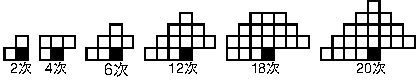
\includegraphics[width=80mm]{fig/fig1.pdf}
   \caption{予測式の形状$p$, 左から$p=0,1,2,3,4,5$とする}
   \label{takago-paper2008080800268-fig:1}
%
   \vspace{2mm}
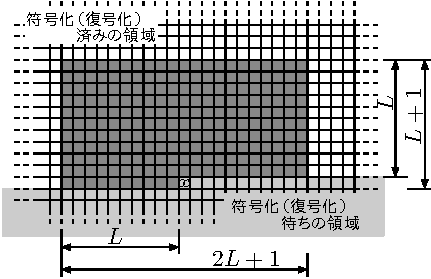
\includegraphics[width=80mm]{fig/fig2.pdf}
\caption{注目画素$x$の予測式係数決定に使われる領域, $L=10,11,\cdots19$とする}
\label{takago-paper2008080800268-fig:2}
   \end{center}
\end{figure}

\begin{table}[t]
\begin{center}
\caption{5種の画像に対する予測誤差のエントロピ}\label{takago-paper2008080800268-tab:1}
\begin{tabular}{lcccc}
\noalign{\hrule height 1pt}
標準画像 & あ & い & え &お\\
\noalign{\hrule height 1pt} 
barbara &4.314&4.331&4.406&4.496\\
        &(4.291)&(4.325)&\\\hline
lenna   &3.913&3.915&3.951&3.956\\
        &(3.890)&(3.909)\\\hline
airplane&4.021&4.027&4.075&4.058\\
        &(3.998)&(4.021)\\\hline
peppers &4.426&4.442&4.491&4.491\\
        &(4.403)&(4.436)\\\hline
girl    &4.368&4.373&4.408&4.442\\
        &(4.345)&(4.367)\\
\noalign{\hrule height 1pt}
\end{tabular}\\
括弧内はオーバーヘッドを含めないときのエントロピ
\end{center}
\end{table}


\begin{thebibliography}{99}
\bibitem{sdkguide}Parrot, ''AR.Drone Developer Guide SDK 2.0''
\end{thebibliography}

\end{document}
